
% extarticle -> kleiner Schriftgrösse
\documentclass[a4paper, 8pt]{extarticle}

%Packages sind in separaten .sty Dateine abgespeichert
\usepackage{include/Vorlage_Cheatsheet}
\usepackage{include/report}
%\usepackage[margin=0.5cm]{geometry}

%\setlist{leftmargin=3mm, nosep}

\title{ZF AEMBS}
\author{Riccardo Degiacomi}
%hello world this is a test for github
%just another test
\begin{document}
% ...stuff goes here....
% 3-column layout
\begin{multicols*}{3}
	\section{SW1 Software und tools}
		\subsection{Design und Architektur}
			\begin{description}
				
				\item[$\bullet$ Mikrocontroller:] Verwendung bei geringem Kosten und Stromverbrauch. Eignet sich für integrierung auf PCB
				\item[$\bullet$ FPGA:] Verwendung wenn mehr Leistung gewünscht als bei $\mu C$ und man Funktionen direkt in HW implementieren möchte (vgl. hoher Stromverbrauch)
				\item[$\bullet$ Embedded Linux:] Verwendung wenn man Netzwerkstacks und Internet nutzen möchte. Bietet grosse Funktionalität. Nachteil; nicht gut für "harte" Echtzeit Anwendungen (langer bootvorgang).
				\item[$\bullet$ Host:] Verwendung bei grossen Systemen. Host ist ähnlich wie PC. Wird oft für GUI und SCADA (Control And Data Acquisition) verwendet.
				
			\end{description}
	Oft werden Systeme als Kombination verschiedener Blöcke Realisiert.\\
	\\
	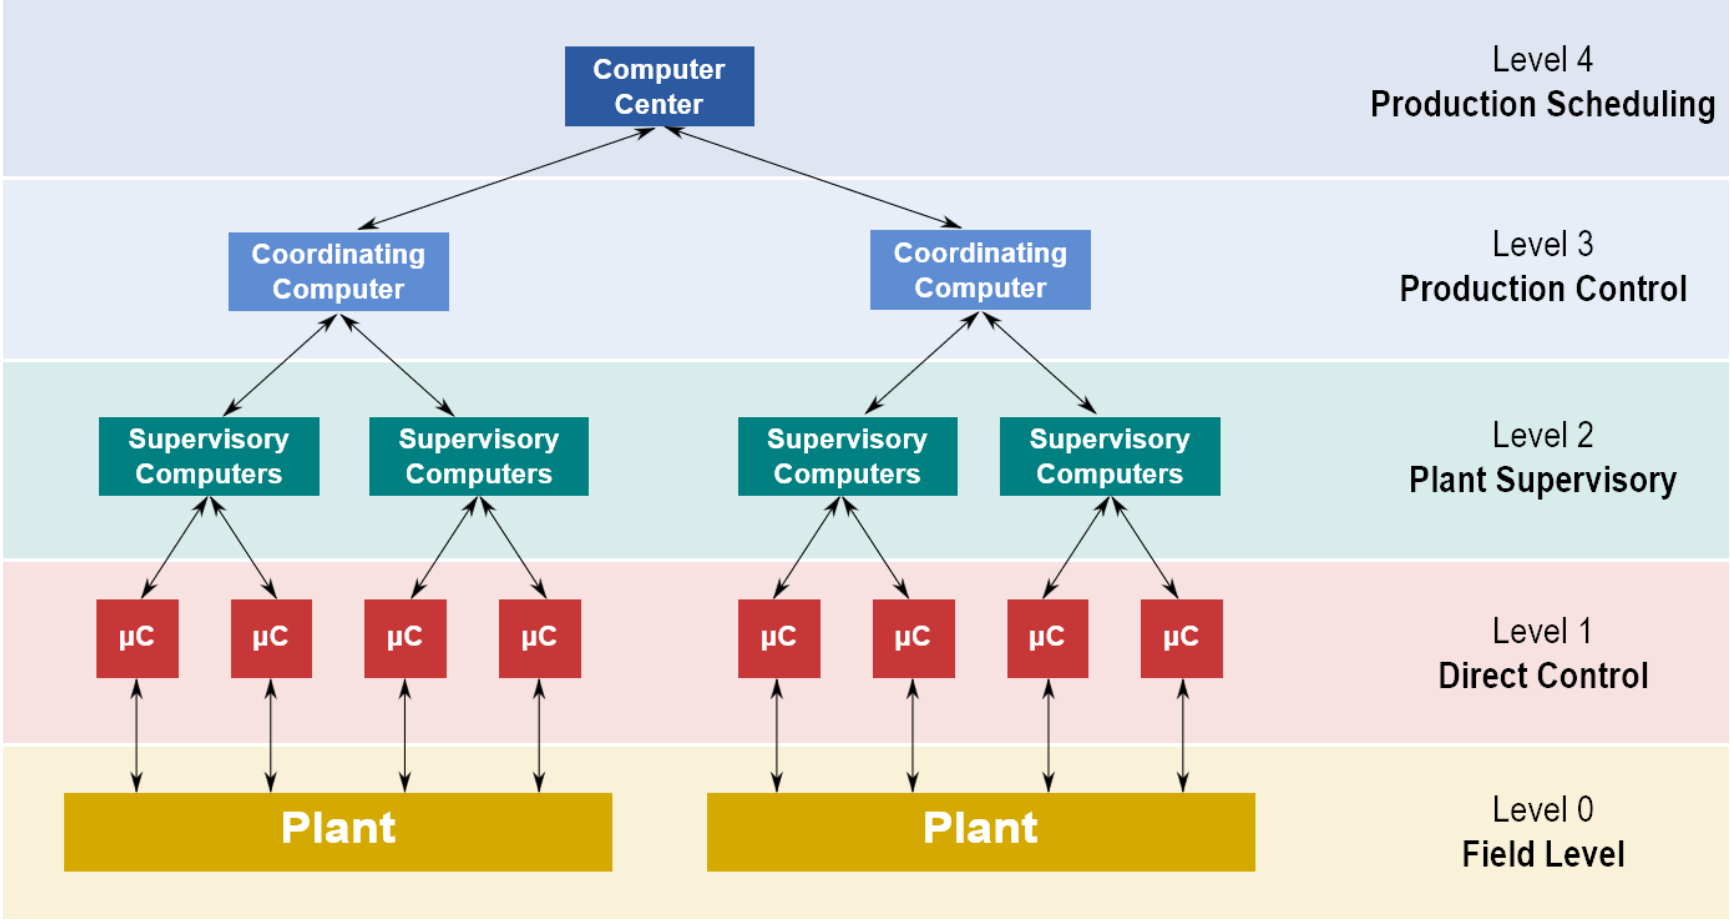
\includegraphics[width=1\linewidth, left]{img/Hardware_Hierarchie}
		\subsection{Crossdevelopment}
		Wenn man nicht auf der selben Entität entwickeln kann spricht man von Host und Target. Auf dem host wird entwickelt, auf dem target ausgeführt. Auf dem Host wird für das Target entwickelt. Dazu nutzt man eine Toolchain.
			\begin{description}
			\item[$\bullet$ Target:] Ist Zielsystem für das entwickelt wird (wofür)
			\item[$\bullet$ Host:] Umgebung auf der entwickelt wird (womit)
			\item[$\bullet$ Toolchain:] Besteht aus Compiler, linker, debugger, standard libraries und anderen Tools
			\item[$\bullet$ Buildumgebung:] Steuert Toolchain und Übersetzungsvorgang. Wird oft mit makefiles gemacht.
			\item[$\bullet$ IDE:] nicht zwingend notwendig\\
			\end{description}

	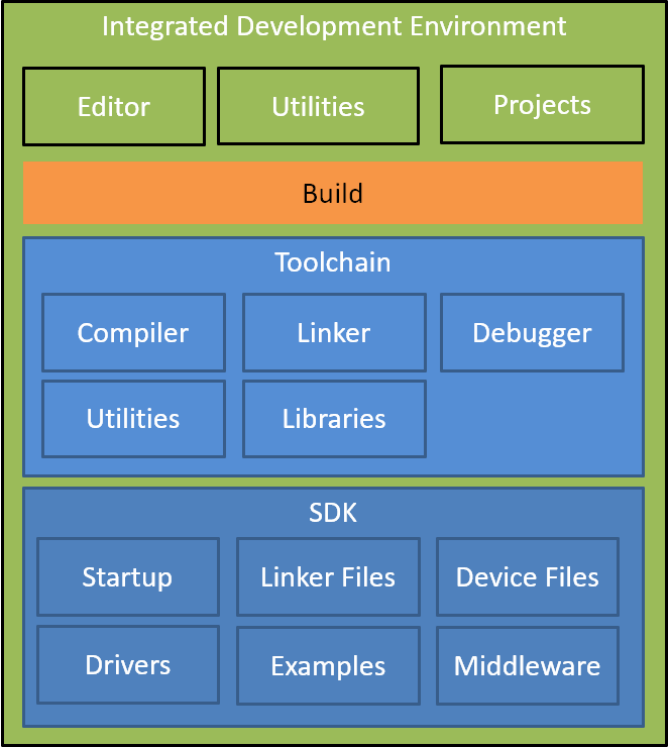
\includegraphics[width=0.9\linewidth,left]{img/Integrated_Development_environement}
		\section{SW2 Software und Device Treiber}
			\subsection{Device Driver}
				\begin{description}
					\item[$\bullet$ Interface:] Abstrahiert von Hardware. Sollte einfach und verständlich sein
					\item[$\bullet$ Synchronisation:] 
					Kann Synchron sein Gadfly, Polling oder asynchron mit Interrupts, Events oder Callbacks (was ist mit snchronisation gemeint dude)
					\item[$\bullet$ Organisation:]
					Einfach: Eine Schnittstellendatei, eine Quelltextdatei (UART,SPI $I^2C$)
					Komplex: Mehrere Dateien mehrere Verzeichnisse  
					\item[$\bullet$ Konfiguration:] Treiber sollte konfigurierbar sein. Gängig ist durch Konfdatei, über Schnittstelle oder mit Makros.
					Siehe:
					https://mcuoneclipse.com/2019/02/23/different-ways-of-software-configuration/
			\end{description}

			\subsection{File Formate}
				\begin{description}
					\item[$\bullet$ ELF/Dwarf:] ist ein Standard Format zur Beschreibung eines ’Executable’
					(Elf) zusammen mit der Debug (Dwarf) Information
					\item[$\bullet$ S19 Motorola S-Record:] Repräsentation der Daten in textueller Form.\\
					Das S19 Format ist ein textuelles und zeilenorientiertes Format, welches
					\colorbox{pink}{’S’ Record ID },\colorbox{yellow}{ Länge },\colorbox{cyan}{ Adresse },\colorbox{green}{ Daten } und eine Checksumme beinhaltet.
					Im Folgenden ein Beispiel:\\
					\colorbox{pink}{S1} \colorbox{yellow}{13} \colorbox{cyan}{7AF0}\\ \colorbox{green}{0A0A0D00000000000000000000000000} 61
					\item[$\bullet$ Intel Hex:]
					Das Intel Hex Format ist auch ein text- und zeilenbasiertes Format, bei
					dem ein Start Code , Länge , Adresse , Typ , Daten und eine Checksumme
					verwendet wird. Nachfolgend auch hier ein Beispiel:\\
					: 10 0100 00 \\214601360121470136007EFE09D21901 40
					\item[$\bullet$ Binary:] Beim Binary Format sind keine zusätzlichen Informationen vorhanden. Bei
					diesem Format sind in der Datei einfach die ’rohen’ Bytes abgespeichert.\newline 
				\end{description}	
	Gemeinsam zu Datei-Formaten von S19, Intel Hex und Binary ist es dass diese
	keine Debug Information enthalten (mussen).\\
	Die benötigen Formate können entweder mit den GNU Werkzeugen direkt
	oder in Eclipse in einem Post-Build Step generiert werden. In der MCUXpresso
	Eclipse IDE können gleich mehrere Formate gleichzeitig in eine Post-Build Step
	erstellt werden
	
		\section{SW3 System}
				\subsection{Systeme}
				%https://www.duden.de/rechtschreibung/integral
				Ein System ist eine Menge von interagierenden oder zusammenhängenden Einheiten, welche ein integrales Ganzes bilden.\\
					\begin{description}
						\item[$\bullet$ Transformierende Systeme:]%beispiel für transformierendes system?
							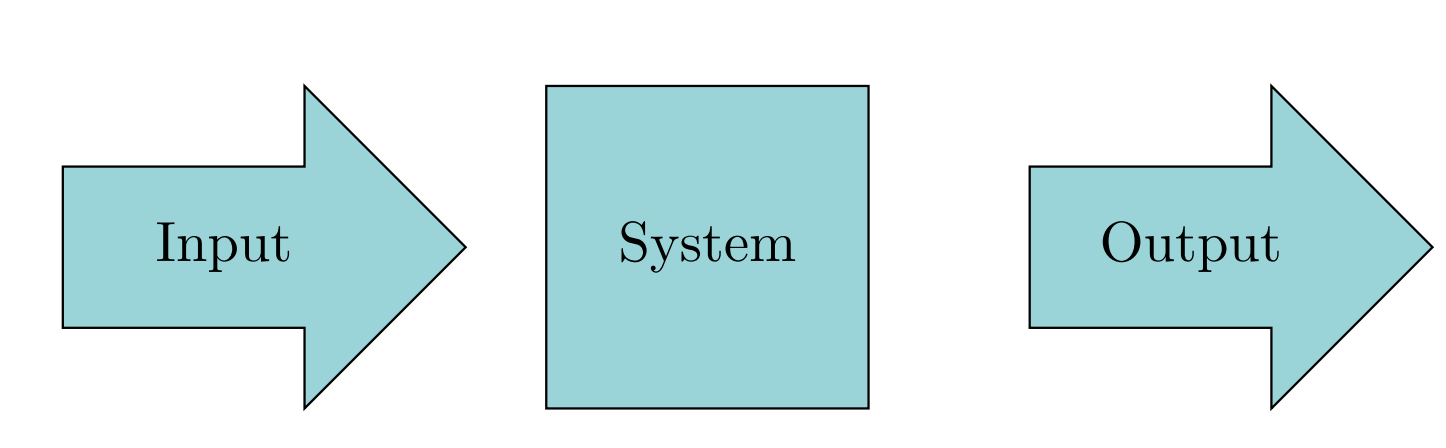
\includegraphics[width=0.8\linewidth,left]{img/Transformierende_Systeme.PNG} 
							Verarbeitet Eingabestrom in Ausgabestrom. Verarbeitet Daten typischer weise kontinuierlich.
							\begin{equation}
								O(s)=P(I(s))
							\end{equation}	
							Dabei ist $I()$ eine Eingabe Funktion, $I(s)$ ein Eingabestrom und $P(s)$ die Systemfunktion. Der Eingabestrom
							wird von der Systemfunktion verarbeitet und erzeugt einen Ausgabestrom $O(s)$. Def. \dq Multichannel System\dq: Ein transformierendes System
							mit mehreren Ein- und Ausgabeströmen. 
							\begin{equation}
								O_m(s)=P(I_n(s)) \qquad m,n \in \mathbb{R}
							\end{equation}
							Eigenschaften: Verarbeitungsqualität (gut oder was?), Durchsatz, Systemausnutzung. Benötigen eine gewisse Menge an Speicher. Optimiert auf
							geringen speicherverbrauch. Konflikt mehr speicher schnellere verarbeitungszeit, aber teurer. Sind oft periodische Systeme (Datenlogger, lesen und verarbeiten Daten mit einer gewissen Periode).
						\item[$\bullet$ Reaktive Systeme:]%bsp?								
							Unterscheiden sich zu transformierenden Systemen dadurch, dass Sie auf Ereignisse warten. Sind typischerweise Steuer- und Regelsysteme.
							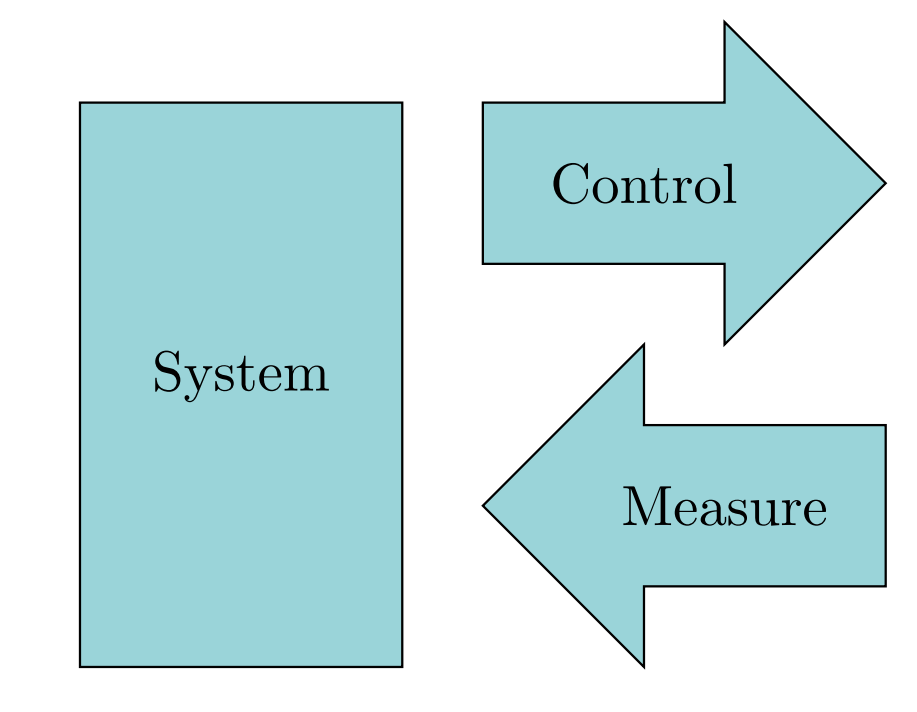
\includegraphics[width=0.6\linewidth,left]{img/Reaktive_Systeme.PNG}
						\item[$\bullet$ Interaktive Systeme:]
							Stellen Schnittstelle zu Benutzer her. Auf kurze Antwortzeit und weil teuer auf hohe auslastung optimiert.
							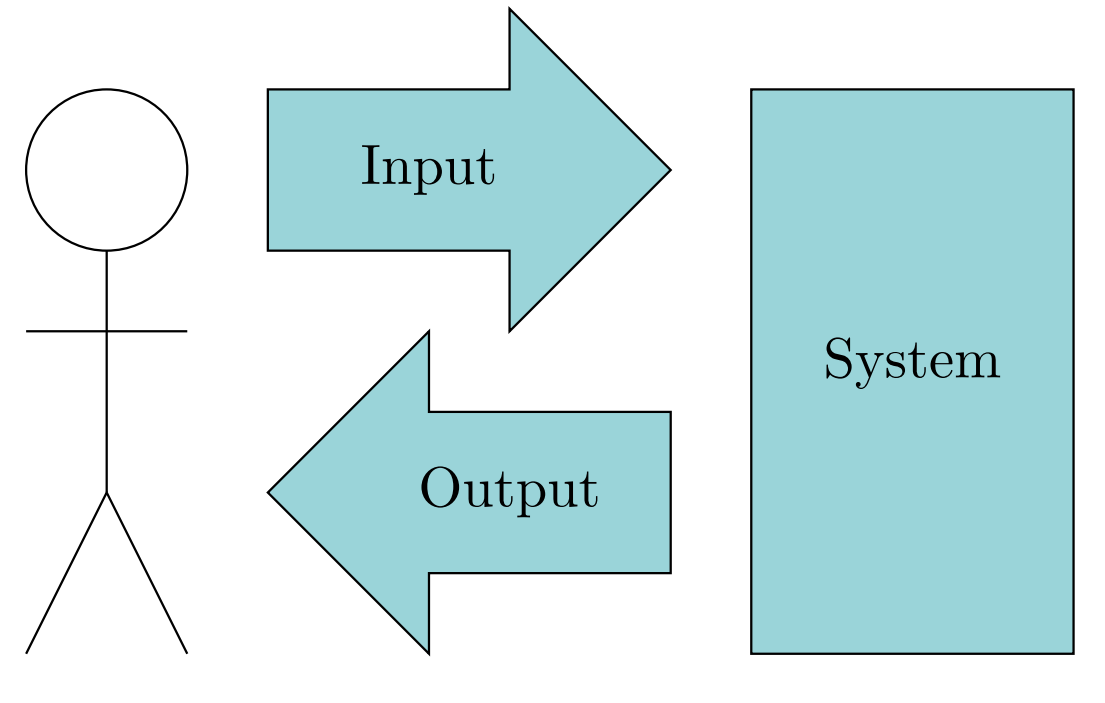
\includegraphics[width=0.6\linewidth,left]{img/Interaktive_Systeme.PNG} 
					\end{description}
		
		\section{Synchronisation}
				
				\subsection{Systeme}
					Computer arbeiten in ihrer eigenen Zeitdomäne. Dies führt zu synchronisationsproblemen mit der Zeitdomäne der echten welt.
					Ein Echtzeitsystem muss die richtige Antwort zur Richtigen Zeit liefern.Timing =  Zeitverhalten, wichtiger Begriff.
					Betrachtet man beispielsweise ein I/O System, stellt man fest, dass dieses nur korrekt funktioniert, wenn Daten zuerst eingelesen und dann gesendet werden.
					Sendet man zu frühm, gehen daten verloren. Um dies zu bewerkstelligen muss man den Ablauf synchronisieren. Es gibt für verschiedene Probleme/Systeme unterschiedliche
					Synchronisationsvarianten.
				\subsection{Handshaking}

				\subsection{Realtime Sync.}
				\subsection{Gadfly Sync.}
				\subsection{Interrupt Sync.}
				\subsection{GPIO Interrupts}

		\section{RTOS}




% ...stuff goes here....

\end{multicols*}



\end{document}